\documentclass[12pt]{article}
%\usepackage[utf8]{inputenc}
\usepackage[margin=1in]{geometry}
\usepackage{amsmath, amssymb}
\usepackage{hyperref, listings}
\usepackage{systeme}
\usepackage{listings}
\usepackage{comment}
\usepackage{enumitem}
%\usepackage[version=4]{mhchem}

\usepackage{enumitem}
\setlist[enumerate,1]{label=(\alph*)}

% Toggle for which version to print
% A bit hacky, there must be a nicer way of doing this...
\usepackage{ifthen}

% Use single counter for problems
\newcounter{ProblemCounter}



\usepackage{pgf,tikz}
\usetikzlibrary{arrows, automata, positioning}
\lstset{numbers=left, numberstyle=\small, numbersep=8pt, frame = single, framexleftmargin=15pt}

\pgfdeclarelayer{nodelayer}
\pgfdeclarelayer{edgelayer}
\pgfsetlayers{edgelayer,nodelayer,main}


% Uncomment next line to compile with solutions
%\def\solutions{1}

\ifx\solutions\undefined
\newcommand{\sol}[1]{}
\else
\newcommand{\sol}[1]{{\color{red} \textbf{Solution: } #1}}
\fi

\ifx\solutions\undefined
\newcommand{\newexampage}{\newpage $\mbox{}$}
\else
\newcommand{\newexampage}{}
\fi

\ifx\solutions\undefined
\newcommand{\examvfill}{\vfill}
\else
\newcommand{\examvfill}{}
\fi


\tikzset{newstyle/.style={thick}}
\tikzset{simple/.style={thick}}

%% PP
\newcommand{\todo}[1]{\vspace{5 mm}\par \noindent \marginpar{\textsc{ToDo}}
\framebox{\begin{minipage}[c]{0.95 \linewidth}
\tt #1 \end{minipage}}\vspace{5 mm}\par}
\newcommand{\R}{{\mathbb R}}
\newcommand{\C}{{\mathbb C}}
\newcommand{\Z}{{\mathbb Z}}
\newcommand{\Q}{{\mathbb Q}}
\newcommand{\N}{{\mathbb N}}
\newcommand{\norm}[1]{\left\lVert#1\right\rVert}
%%
%% CY
\newcommand{\bmat}[1]{\begin{bmatrix}#1\end{bmatrix}}
\newcommand{\abs}[1]{\left| #1 \right|}
\newcommand{\dotp}[1]{\left\langle #1 \right\rangle}
\DeclareMathOperator{\rank}{rank}
\DeclareMathOperator{\proj}{proj}
\DeclareMathOperator{\spann}{span}
%%


\title{18.C21 Midterm \\
Spring 2026 (Johnson \& Marzouk)
\ifdefined\solutions
--- \textcolor{red}{Solutions}
\fi
}
\author{}
\date{}
\begin{document}

\maketitle

\ifx\solutions\undefined

% Signature line
{\vspace{0.5cm} \hspace{1cm}
{\Large \textbf{NAME:} \dotfill}
\hspace{2cm}\ \vspace{0.5cm}}

\fi

\begin{itemize}

\item You have \textbf{50 minutes}.  \textbf{Please allocate your time carefully}, to make sure you get to work on all parts---take a quick look at the \emph{whole exam} before starting.

\item Write your \textbf{NAME} above \emph{and} at the top of \emph{every} page. Please do it as soon as you begin the exam, and check again before returning it. 

\item Only write on \emph{one} side of each sheet.  Additional paper will be provided upon request.

\item You can bring \textbf{1 letter-sized sheet of notes} (both sides if you want).

\item \textbf{Show your work / justify your answers.}  Wrong answers may still receive partial credit \emph{if} the reasoning was somewhat correct.

\item If you absolutely believe there is something wrong with a problem, please ask. No hints, other than the ones already written in the exam, will be given.

%\item Once you are done, or the \textbf{2-hour exam time} is up, please upload your file in \textbf{Gradescope}. Again, please make sure you write your name in every page.

\end{itemize}

\subsection*{A few useful formulas and facts from class}
\begin{itemize}
    \item Double-precision (\texttt{Float64}) floating-point numbers store about 15--16 decimal significant digits, and can represent magnitudes from around $\approx 10^{-300}$ to around $\approx 10^{300}$ (after which they under/overflow, respectively).
    \item A least-square problem $\min_x \Vert Ax - b \Vert_2$ is minimized when $A^T A x = A^T b$.
    \item The Chebyshev points for polynomial interpolation on $[-1,1]$ are $x_k = \cos(k\pi/n)$ for $k=0,\ldots,n$.
    \item A Newton step for $f(x)=0$ is $x_{k+1} = x_k - f'(x_k)^{-1} f(x_k)$.
    \item Piecewise-linear interpolation with intervals $\Delta x$ has an error $O(\Delta x^2)$ for twice-differentiable functions.
    \item Polynomial interpolation from Chebyshev points, and resulting algorithms like Clenshaw--Curtis quadrature, converges exponentially fast for any function with a Taylor series (or at least faster than any power law if the function is infinitely differentiable).
\end{itemize}

%%%%%%%%%%%%%%%%%%%%%%%%%%%%%%%%%%%%%%%%%%%%%%%%%%%%%%%%%

\newpage
\section*{Problem 1 (10+10 points)}

The roots $x_1,x_2$ of a quadratic equation $ax^2 + bx +c =0$ can be found from the quadratic formula, but these solutions can be written in a different form by instead solving $a + bx^{-1} + cx^{-2}=0$ for $x^{-1}$, resulting in two possible expressions for each root:
\begin{align*}
x_1 &= \frac{-b + \sqrt{b^2 - 4ac}}{2a} = \frac{2c}{-b - \sqrt{b^2 - 4ac}} \, , \\
x_2 &= \frac{-b - \sqrt{b^2 - 4ac}}{2a} = \frac{2c}{-b + \sqrt{b^2 - 4ac}} \, .
\end{align*}
Call the formula on the left the ``regular'' formula and the one on the right the ``inverted'' formula.
\begin{enumerate}
    \item For a particular choice of $a,b,c$, you find that the ``inverted'' formula for $x_1$ is \emph{much} more accurate than the ``regular'' formula in double/\texttt{Float64} precision.  Give example values of $a,b,c$ where that would be true.  Also, which of the two formulas for $x_2$ will be more accurate in this case?

    \item You find in \texttt{Float64} precision that the regular formula for $x_1$ is giving \texttt{Inf} and the inverted formula for $x_1$ is giving \texttt{0.0}, but none of $a,b,c$ are \texttt{Inf} or \texttt{0.0}, and an arbitrary precision calculation tells you that the correct answer for $x_1$ should be nonzero and representable as a finite value in \texttt{Float64} precision.   Give example values of $a,b,c$ where this might be happening, and explain how to correct the formulas to handle this case accurately while staying in \texttt{Float64} precision.
\end{enumerate}

\sol{
\begin{enumerate}
    \item For one to be much more accurate than the other, a likely explanation is that $-b + \sqrt{b^2 - 4ac}$ experienced \textbf{catastrophic cancellation} while $-b - \sqrt{b^2 - 4ac}$ did not.  That occurs when the former expression is a \emph{subtraction of nearly equal quantities} and the latter is an \emph{addition}.   $-b + \sqrt{b^2 - 4ac}$ being a subraction requires $\boxed{b > 0}$, and the quantities being nearly equal requires $\boxed{|4ac| \ll b^2}$.  There are many possible values for which this is true, but one example would be:
    $$
    a = b = 1 \text{ and } c \approx 10^{-20} \, .
    $$
    In this case the regular formula will give $x_1 = 0$ (which has \emph{no} correct digits) since $b^2 \ominus 4ac = b^2$, whereas the second formula will give $x_1 \approx 2c/(-b - b) = -c/b \approx 10^{-20}$. In that case you would use the \textbf{regular formula for $x_2$} for the same reason: to make sure you \emph{add} two quantities of the same sign rather than subtracting.
    
    \item A likely explanation here is that either $b^2$ or $4ac$ \textbf{overflowed}, e.g. $\boxed{a=c=1 \text{ and } b \approx 10^{200}}$.   A simple fix in this case would be to pull a factor of $|b|$ out of the square root, i.e.~replace $\sqrt{b^2-4ac} = \boxed{|b| \sqrt{1 - 4ac/b^2}}$ in both formulas.  Similarly, if $a$~and/or~$c$ is huge e.g.~$\boxed{b=1 \text{ and } a = -c \approx 10^{200}}$, you could factor out $\sqrt{|a|}$ and/or $\sqrt{|c|}$.

    As in the previous part, you would also want to choose the correct formula if $|4ac| \ll b^2$: the $-b + |b|\sqrt{\cdots}$ formulas if $b>0$ and the $-b - |b|\sqrt{\cdots}$ formulas if $b < 0$.

    Another possible solution that works if $ac < 0$, and which handles overflow in either $ac$ or $b^2$, is to factor
    $$
    \sqrt{b^2-4ac} = \sqrt{|b|-2\sqrt{|a|}\sqrt{|c|}} \sqrt{|b| +2\sqrt{|a|}\sqrt{|c|}} \, ,
    $$
    computed in the order indicated by the square roots, so that we always take square roots \emph{before|} multiplying.  (If $ac > 0$ then you would need to replace $2$ with $2i$ in the above expression, using complex numbers.  But in general with complex numbers you may need to be careful of branch cuts, and it's a bit outside the scope of the course.  Languages like Julia or Python will not take complex square roots of negative numbers unless you explicitly request it.)
\end{enumerate}
}
\examvfill

\newexampage
\newexampage

\section*{Problem 2 (10 points)}

Suppose that you are given a function value $f(x_1)$ and $f(x_2)$ at two points $x_1, x_2$ and are also given the \emph{derivative} $f'(x_1)$ and $f'(x_2)$ at those two points.

Explain how to find a polynomial interpolant $p(x)$ that matches \emph{both} $f$ and $f'$ at $x_1,x_2$.  What should the degree of $p(x)$ be?  Write down a system of linear equations for the coefficients of $p$.  (You don't need to solve them.)


\sol{

We will have \textbf{four equations} (two constraints on $p$ and two on $p'$), so we need four unknowns, and hence a \textbf{degree-3 polynomial} $p(x) = c_0 + c_1 x + c_2 x^2 + c_3 x^3$ (and hence $p' = c_1 + 2 c_2x + 3c_3 x^2$).

The four equations will be
$$
\begin{pmatrix}
p(x_1) \\
p(x_2) \\
p'(x_1) \\
p'(x_2)
\end{pmatrix} =
\boxed{
\begin{pmatrix}
1 & x_1 & x_1^2 & x_1^3 \\
1 & x_2 & x_2^2 & x_2^3 \\
0 & 1 & 2x_1 & 3x_1^2 \\
0 & 1 & 2x_2 & 3x_2^2 
\end{pmatrix}
\begin{pmatrix}
c_0 \\
c_1 \\
c_2 \\
c_3
\end{pmatrix}
= \begin{pmatrix}
f(x_1) \\
f(x_2) \\
f'(x_1) \\
f'(x_2)
\end{pmatrix}
} \, ,
$$
which is a $4\times 4$ system of equations that is solvable if $x_1 \ne x_2$.

}
\examvfill


\newpage

%%%%%%%%%%%%%%%

\section*{Problem 3 (10+10 points)}

Suppose that you are trying to compute
$$
I = \int_0^2 \left| f(x) \right| \, dx \, .
$$
where
$$
f(x) = \sin(x - \cos(x)) \, ,
$$
and the integrand $|f(x)|$ is plotted in Fig.~\ref{fig:kinkyintegrand} below along with $f(x)$.
\begin{figure}[b!]
    \centering
    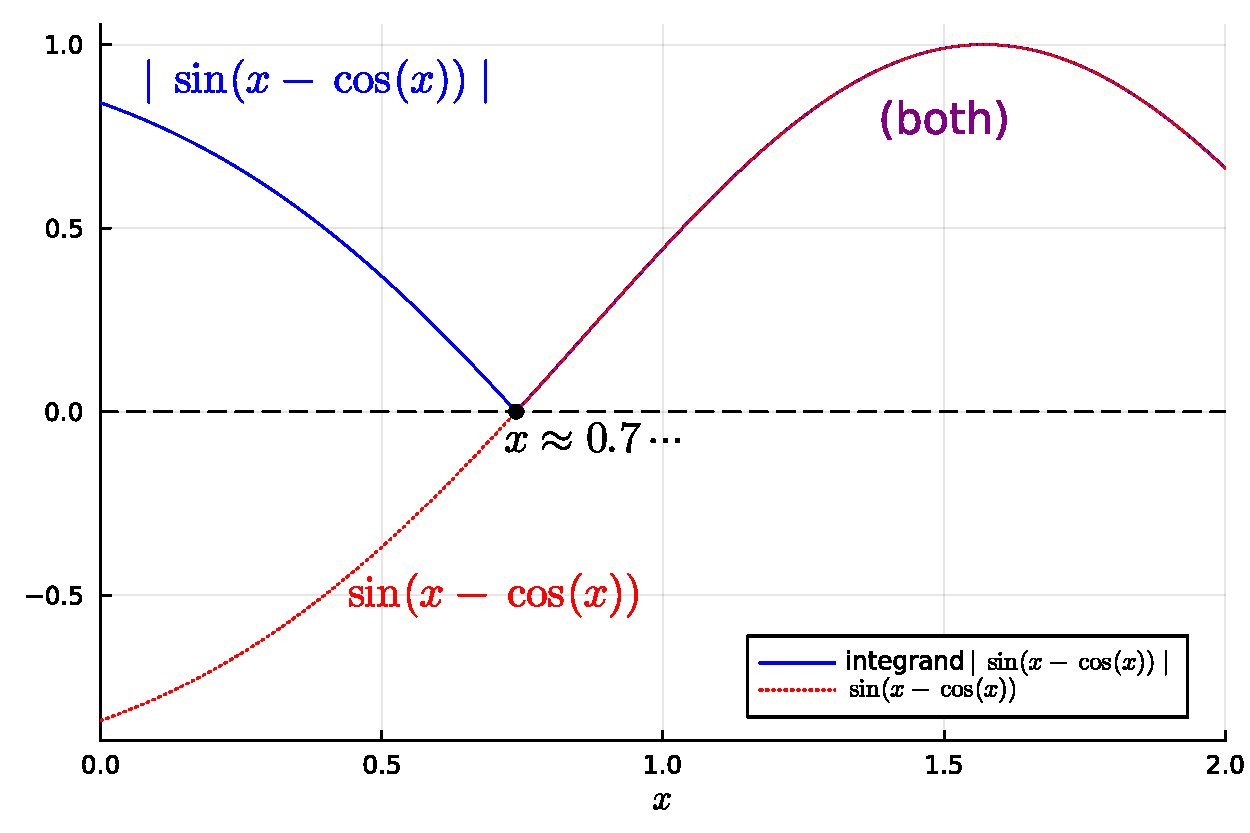
\includegraphics[width=0.7\textwidth]{kinkyintegrand.pdf}
    \caption{Plot of the integrand $|f(x)| = \left| \sin(x - \cos(x)) \right|$ (blue line) along with the function $f(x) = \sin(x - \cos(x))$ without the absolute value (red dotted).  The zero crossing (black dot) occurs at an irrational $x$ that is $\approx 0.7\cdots$.}
    \label{fig:kinkyintegrand}
\end{figure}

\begin{enumerate}
    \item If you estimated this integral using the trapezoidal rule with $n + 1$ equispaced points ($n$ intervals), what would you expect the convergence rate to be? For example, is the error $O(1/n^2), O(1/n^{1.5}), O(1/n),\ldots$?  Justify your answer (briefly).

    \item Outline an algorithm to get $I$ with exponentially fast convergence using Clenshaw--Curtis quadrature and \emph{some other ingredient}.  (Assume you have a subroutine \texttt{$I_n$ = clencurt(func,a,b,n)} that estimates the integral $\int_a^b\text{func}(x)dx$ of any given function $\texttt{func}$ by Clenshaw--Curtis quadrature on any given interval $[a,b]$ and for any number of points $n+1$; you need not outline the Clenshaw--Curtis algorithm itself.)  Why is Clenshaw--Curtis \emph{alone} not enough here?
\end{enumerate}

\newpage $\mbox{}$
\sol{

\begin{enumerate}
\item The error should converge as $\boxed{O(1/n^2)} = O(\Delta x^2)$.  We saw in class that the trapezoidal rule converges as $O(\Delta x^2)$ in the regions where the integrand is smooth, because piecewise-linear approximation converges at this rate.  However, around the ``kink'' when $f(x)=0$, the derivative is discontinuous, and we saw in pset~1 that piecewise-linear interpolation only converges as $O(\Delta x)$ in this case.  However, this is only \emph{one interval}, and so the contribution to the \emph{area} from that one interval is proportional to the error in the function multiplied by $\Delta x$, and hence the ``kink'' contributes a $O(\Delta x^2)$ error.

\item Clenshaw--Curtis alone is not enough here because \textbf{the integrand is not smooth}, which will spoil the exponential convergence.  In fact, a deeper analysis (from the convergence of a Fourier cosine series for a function with a derivative discontinuity, which can be analyzed by integration-by-parts as in class) shows that it should have only $O(1/n^2)$ convergence, the same as the trapezoidal rule, but you were not required to be this precise.

The solution is to just \textbf{break the integral into two pieces at the root} $x_*$ where $f(x_*)=0$: apply Clenshaw--Curtis quadrature \emph{separately} to each term in 
$$
I = \int_0^{x_*} \left| f(x) \right| \, dx  + \int_{x_*}^2 \left| f(x) \right| \, dx\, = -\int_0^{x_*}  f(x) \, dx  + \int_{x_*}^2  f(x) \, dx\, .
$$
If we use order-$n$ quadrature for each piece, it will converge at least exponentially fast for each piece and hence exponentially fast overall.

However, we don't know the root exactly---it occurs when $\sin(x-\cos(x)) = 0$ (or equivalently when $x - \cos(x) = 0$ in this case), which is a transcendental equation with an irrational solution that cannot be written in closed form.  Fortunately, we can easily \textbf{find the root $x_*$ with a Newton iteration}
$$
x_{k+1} = x_k - \frac{f(x_k)}{f'(x_k)} = x_k - \frac{\tan(x_k - \cos x_k)}{1 + \sin(x_k)} \, ,
$$
with some starting guess, e.g.~$x_1 = 0.7$ from the plot.  (You could also alternatively Newton's method to solve $x - \cos(x) = 0$.)

This will very quickly converge to any desired precision, e.g.~if you converge it to nearly machine precision then it won't be the limiting factor in the Clenshaw--Curtis integration.   Obviously, you can't carry out the Newton iteration on the exam, but, if you did, you would find that the first few iterations (in arbitrary precision) are
\begin{align*}
x_1 &= \mathbf{0.7}\\
x_2 &= \mathbf{0.739}491861\ldots \\
x_3 &= \mathbf{0.7390851}69664\ldots \\
x_4 &= \mathbf{0.739085133215160}935\ldots \\
x_5 &= \mathbf{ 0.7390851332151606416553120876738}924\ldots
\, ,
\end{align*}
where the correct digits are shown in bold: we only need 3--4 steps in \texttt{Float64}!
\end{enumerate}
}

\newexampage

\end{document}
